\documentclass[10pt,aspectratio=169]{beamer}

% Theme and colors
\usetheme{Madrid}
\usecolortheme{whale}
\setbeamertemplate{navigation symbols}{}
\setbeamertemplate{footline}[frame number]

% Packages
\usepackage[utf8]{inputenc}
\usepackage[T1]{fontenc}
\usepackage{amsmath,amssymb,amsthm}
\usepackage{mathtools}
\usepackage{booktabs}
\usepackage{graphicx}
\usepackage{tikz}
\usepackage{pgfplots}
\pgfplotsset{compat=1.17}
\usepackage{algorithm}
\usepackage{algorithmic}
\usepackage{multirow}
\usepackage{colortbl}
\usepackage{xcolor}

% Custom colors
\definecolor{darkblue}{RGB}{0,51,102}
\definecolor{lightblue}{RGB}{230,240,250}
\definecolor{darkgreen}{RGB}{0,100,0}
\definecolor{darkred}{RGB}{139,0,0}

% Title information
\title[Time-Varying Factor Allocation]{\textbf{Time-Varying Factor Allocation}}
\subtitle{Replication of Vincenz \& Zeissler (2022)}
\author{Thomas Betton}
\institute{Universit\'e Paris-Dauphine \\ Master Gestion Quantitative}
\date{\today}

\begin{document}

% ============================================================================
% TITLE PAGE
% ============================================================================
\begin{frame}
    \titlepage
\end{frame}

% ============================================================================
% TABLE OF CONTENTS
% ============================================================================
\begin{frame}{Plan de la pr\'esentation}
    \tableofcontents
\end{frame}

% ============================================================================
% SECTION 1: INTRODUCTION
% ============================================================================
\section{Introduction et Contexte}

\begin{frame}{Objectif de l'\'etude}
    \begin{block}{Question de recherche}
        Peut-on am\'eliorer la performance d'un portefeuille de facteurs en utilisant des variables macro\'economiques pour pr\'edire les rendements futurs?
    \end{block}

    \vspace{0.5cm}

    \textbf{Approche m\'ethodologique:}
    \begin{enumerate}
        \item Construction de \textbf{21 facteurs} sur 4 classes d'actifs
        \item \textbf{R\'egression bay\'esienne pr\'edictive} avec prior conservateur
        \item Allocation \textbf{Black-Litterman} avec contrainte de tracking error
        \item Analyse de \textbf{15 variables pr\'edictives}
    \end{enumerate}

    \vspace{0.3cm}

    \begin{alertblock}{R\'esultat principal du papier}
        9/15 strat\'egies significatives \`a 5\%, dont 8 survivent la correction de Holm-Bonferroni
    \end{alertblock}
\end{frame}

\begin{frame}{Classes d'actifs et facteurs}
    \begin{table}[h]
        \centering
        \small
        \begin{tabular}{lcccc}
            \toprule
            \textbf{Style} & \textbf{FX} & \textbf{Commodities} & \textbf{Fixed Income} & \textbf{Equities} \\
            \midrule
            Market & \checkmark & \checkmark & \checkmark & \checkmark \\
            Carry & \checkmark & \checkmark & \checkmark & -- \\
            Momentum & \checkmark & \checkmark & \checkmark & \checkmark \\
            Value & \checkmark & \checkmark & \checkmark & \checkmark \\
            Size & -- & -- & -- & \checkmark \\
            Basis-Momentum & -- & \checkmark & -- & -- \\
            \midrule
            \textbf{Total} & 4 & 5 & 4 & 4 \\
            \bottomrule
        \end{tabular}
        \caption{Distribution des 17 facteurs impl\'ement\'es}
    \end{table}

    \begin{itemize}
        \item Chaque facteur est \textbf{volatility-scaled} \`a 10\% annualis\'e
        \item Portefeuilles long-short bas\'es sur le tri en \textbf{sextiles} (top/bottom 16.67\%)
    \end{itemize}
\end{frame}

% ============================================================================
% SECTION 2: CONSTRUCTION DES FACTEURS
% ============================================================================
\section{Construction des Facteurs}

\begin{frame}{Facteur Momentum (12-1)}
    \begin{block}{D\'efinition math\'ematique}
        Signal de momentum pour l'actif $i$ au temps $t$:
        \begin{equation}
            \text{Mom}_{i,t} = \prod_{k=2}^{12} (1 + r_{i,t-k}) - 1
        \end{equation}
        o\`u $r_{i,t-k}$ est le rendement mensuel de l'actif $i$ au mois $t-k$.
    \end{block}

    \vspace{0.3cm}

    \textbf{Construction du portefeuille:}
    \begin{enumerate}
        \item Classer les actifs par signal de momentum
        \item \textbf{Long}: Top sextile (16.67\% des actifs avec le plus haut momentum)
        \item \textbf{Short}: Bottom sextile (16.67\% avec le plus bas momentum)
        \item Pond\'eration \'egale au sein de chaque groupe
    \end{enumerate}

    \begin{equation}
        r_{\text{Mom},t+1} = \sum_{i \in \text{Top}} w_i \cdot r_{i,t+1} - \sum_{i \in \text{Bottom}} w_i \cdot r_{i,t+1}
    \end{equation}
\end{frame}

\begin{frame}{Facteur Carry}
    \textbf{FX Carry} - Bas\'e sur les diff\'erentiels de taux d'int\'er\^et:
    \begin{equation}
        \text{Carry}_{i,t}^{FX} = r_{i,t}^{foreign} - r_{t}^{USD}
    \end{equation}

    \vspace{0.3cm}

    \textbf{Commodity Carry} - Bas\'e sur le roll yield:
    \begin{equation}
        \text{Carry}_{i,t}^{Commo} = \frac{F_{i,t}^{(1)} - F_{i,t}^{(2)}}{F_{i,t}^{(2)}}
    \end{equation}
    o\`u $F^{(1)}$ et $F^{(2)}$ sont les prix des contrats front et second month.

    \vspace{0.3cm}

    \textbf{Fixed Income Carry} - Bas\'e sur le niveau des taux:
    \begin{equation}
        \text{Carry}_{i,t}^{FI} = y_{i,t}^{10Y}
    \end{equation}

    \begin{alertblock}{Interpr\'etation}
        Carry \'elev\'e $\Rightarrow$ Position longue (prime de risque positive attendue)
    \end{alertblock}
\end{frame}

\begin{frame}{Facteur Value}
    \begin{block}{Signal de Value}
        D\'eviation par rapport \`a la moyenne mobile 5 ans:
        \begin{equation}
            \text{Value}_{i,t} = \frac{\bar{P}_{i,t}^{60M}}{P_{i,t}} - 1
        \end{equation}
        o\`u $\bar{P}_{i,t}^{60M} = \frac{1}{60}\sum_{k=0}^{59} P_{i,t-k}$
    \end{block}

    \vspace{0.3cm}

    \textbf{Interpr\'etation:}
    \begin{itemize}
        \item Value positif $\Rightarrow$ Prix actuel inf\'erieur \`a la moyenne historique
        \item Actif potentiellement \textbf{sous-\'evalu\'e}
        \item Esp\'erance de \textbf{mean reversion}
    \end{itemize}

    \vspace{0.3cm}

    \textbf{Variantes par classe d'actifs:}
    \begin{itemize}
        \item \textbf{FX}: D\'eviation PPP (Purchasing Power Parity)
        \item \textbf{Equities}: Price-to-Book, Earnings Yield
        \item \textbf{Commodities}: D\'eviation du prix spot
    \end{itemize}
\end{frame}

\begin{frame}{Volatility Scaling}
    \begin{block}{Objectif}
        Normaliser tous les facteurs \`a une volatilit\'e cible de \textbf{10\% annualis\'e} pour assurer la comparabilit\'e.
    \end{block}

    \textbf{M\'ethodologie:}
    \begin{equation}
        r_{f,t}^{scaled} = r_{f,t} \times \frac{\sigma_{target}}{\hat{\sigma}_{f,t-1}}
    \end{equation}

    o\`u:
    \begin{itemize}
        \item $\sigma_{target} = 10\%$ (annualis\'e)
        \item $\hat{\sigma}_{f,t-1}$ = volatilit\'e estim\'ee sur fen\^etre glissante de 36 mois
    \end{itemize}

    \vspace{0.3cm}

    \textbf{Contraintes de leverage:}
    \begin{equation}
        \text{Scale}_{f,t} = \min\left(3.0, \max\left(0.1, \frac{\sigma_{target}}{\hat{\sigma}_{f,t-1}}\right)\right)
    \end{equation}

    \begin{alertblock}{Importance}
        Sans scaling, les facteurs haute volatilit\'e domineraient le portefeuille
    \end{alertblock}
\end{frame}

% ============================================================================
% SECTION 3: VARIABLES PREDICTIVES
% ============================================================================
\section{Variables Pr\'edictives}

\begin{frame}{Les 15 Variables Pr\'edictives}
    \begin{table}[h]
        \centering
        \scriptsize
        \begin{tabular}{llc}
            \toprule
            \textbf{Cat\'egorie} & \textbf{Variable} & \textbf{Disponibilit\'e} \\
            \midrule
            \multirow{4}{*}{Macro\'economie} & CFNAI (Chicago Fed National Activity) & \checkmark \\
            & Inflation (CPI YoY) & \checkmark \\
            & Short Rate (3M T-Bill) & \checkmark \\
            & Budget Balance & Limit\'e \\
            \midrule
            \multirow{3}{*}{Courbe des taux} & Yield Curve (10Y - 2Y) & \checkmark \\
            & TED Spread & Non disponible \\
            & M2 Growth & \checkmark \\
            \midrule
            \multirow{3}{*}{Volatilit\'e/Risque} & VIX & \checkmark \\
            & SKEW & \checkmark \\
            & EPU (Economic Policy Uncertainty) & \checkmark \\
            \midrule
            \multirow{2}{*}{Factor-based} & TS Momentum & \checkmark \\
            & TS Volatility & \checkmark \\
            \bottomrule
        \end{tabular}
    \end{table}

    \begin{alertblock}{Probl\`eme de donn\'ees}
        TED Spread: ``\#N/A Invalid Security'' $\Rightarrow$ Aucune donn\'ee valide
    \end{alertblock}
\end{frame}

\begin{frame}{Standardisation des Pr\'edicteurs}
    \begin{block}{Transformation z-score avec fen\^etre expansive}
        \begin{equation}
            z_{t} = \frac{x_t - \bar{x}_{1:t}}{\hat{\sigma}_{1:t}}
        \end{equation}
        o\`u $\bar{x}_{1:t}$ et $\hat{\sigma}_{1:t}$ sont calcul\'es sur toutes les observations jusqu'\`a $t$.
    \end{block}

    \vspace{0.3cm}

    \textbf{Avantages de la fen\^etre expansive:}
    \begin{itemize}
        \item \'Evite le \textbf{look-ahead bias}
        \item Estimation plus stable au fil du temps
        \item Coh\'erent avec l'information disponible en temps r\'eel
    \end{itemize}

    \vspace{0.3cm}

    \textbf{P\'eriode minimale requise:} 120 mois (10 ans) avant de g\'en\'erer des pr\'edictions.
\end{frame}

% ============================================================================
% SECTION 4: REGRESSION BAYESIENNE
% ============================================================================
\section{R\'egression Bay\'esienne Pr\'edictive}

\begin{frame}{Motivation: Pourquoi Bay\'esien?}
    \textbf{Probl\`eme du sur-ajustement:}
    \begin{itemize}
        \item Les rendements financiers ont un faible ratio signal/bruit
        \item OLS tend \`a \textbf{sur-estimer} la pr\'edictabilit\'e
        \item R\'esultat: mauvaise performance out-of-sample
    \end{itemize}

    \vspace{0.5cm}

    \begin{block}{Solution Bay\'esienne}
        Imposer un \textbf{prior conservateur} qui shrink les estimations vers z\'ero:
        \begin{equation}
            \text{Prior: } R^2 < 1\%
        \end{equation}
    \end{block}

    \vspace{0.3cm}

    \textbf{Interpr\'etation:}
    \begin{itemize}
        \item A priori, nous croyons que la pr\'edictabilit\'e est tr\`es faible
        \item Les donn\'ees doivent \^etre tr\`es convaincantes pour modifier cette croyance
        \item R\'esultat: pr\'edictions plus \textbf{robustes} et \textbf{r\'ealistes}
    \end{itemize}
\end{frame}

\begin{frame}{Mod\`ele de R\'egression}
    \begin{block}{Mod\`ele lin\'eaire}
        \begin{equation}
            r_{f,t+1} = \alpha + \beta \cdot z_t + \varepsilon_{t+1}
        \end{equation}
        o\`u $r_{f,t+1}$ est le rendement du facteur $f$ et $z_t$ le pr\'edicteur standardis\'e.
    \end{block}

    \vspace{0.3cm}

    \textbf{Estimation OLS:}
    \begin{equation}
        \hat{\beta}_{OLS} = \frac{\sum_{s=1}^{t} (z_s - \bar{z})(r_{f,s+1} - \bar{r}_f)}{\sum_{s=1}^{t} (z_s - \bar{z})^2}
    \end{equation}

    \textbf{Variance r\'esiduelle:}
    \begin{equation}
        \hat{\sigma}^2 = \frac{1}{t-2} \sum_{s=1}^{t} (r_{f,s+1} - \hat{\alpha} - \hat{\beta}_{OLS} \cdot z_s)^2
    \end{equation}
\end{frame}

\begin{frame}{Shrinkage Bay\'esien}
    \begin{block}{Prior sur $\beta$}
        \begin{equation}
            \beta \sim \mathcal{N}\left(0, \sigma_\beta^2\right) \quad \text{avec} \quad \sigma_\beta^2 = \frac{R^2_{prior} \cdot \text{Var}(r_f)}{\text{Var}(z)}
        \end{equation}
    \end{block}

    \textbf{Formule du posterior:}
    \begin{equation}
        \hat{\beta}_{Bayes} = \frac{\tau_{OLS}}{\tau_{OLS} + \tau_{prior}} \cdot \hat{\beta}_{OLS}
    \end{equation}

    o\`u:
    \begin{itemize}
        \item $\tau_{OLS} = \frac{\sum(z - \bar{z})^2}{\hat{\sigma}^2}$ (pr\'ecision OLS)
        \item $\tau_{prior} = \frac{1}{\sigma_\beta^2}$ (pr\'ecision prior)
    \end{itemize}

    \vspace{0.3cm}

    \begin{alertblock}{Shrinkage Factor}
        \begin{equation}
            \text{Shrinkage} = \frac{\tau_{OLS}}{\tau_{OLS} + \tau_{prior}} \in [0, 1]
        \end{equation}
        Avec $R^2_{prior} = 1\%$, le shrinkage typique est de $\approx 0.78$
    \end{alertblock}
\end{frame}

\begin{frame}{Algorithme de Pr\'ediction}
    \begin{algorithm}[H]
        \scriptsize
        \caption{Bayesian Predictive Regression}
        \begin{algorithmic}[1]
            \REQUIRE Rendements $\{r_{f,s}\}_{s=1}^T$, Pr\'edicteur $\{z_s\}_{s=1}^T$, Prior $R^2 = 0.01$
            \ENSURE Pr\'edictions $\{\hat{r}_{f,t+1}\}_{t=60}^{T-1}$
            \FOR{$t = 60$ \TO $T-1$}
                \STATE Estimer $\hat{\beta}_{OLS}$ et $\hat{\sigma}^2$ sur $\{1, \ldots, t\}$
                \STATE Calculer $\sigma_\beta^2 = R^2_{prior} \cdot \text{Var}(r_f) / \text{Var}(z)$
                \STATE Calculer $\tau_{OLS}$ et $\tau_{prior}$
                \STATE $\hat{\beta}_{Bayes} \leftarrow \frac{\tau_{OLS}}{\tau_{OLS} + \tau_{prior}} \cdot \hat{\beta}_{OLS}$
                \STATE $\hat{\alpha}_{Bayes} \leftarrow \bar{r}_f$
                \STATE $\hat{r}_{f,t+1} \leftarrow \hat{\alpha}_{Bayes} + \hat{\beta}_{Bayes} \cdot (z_t - \bar{z})$
            \ENDFOR
        \end{algorithmic}
    \end{algorithm}

    \vspace{0.3cm}

    \textbf{Points cl\'es:}
    \begin{itemize}
        \item Estimation \textbf{out-of-sample} (expanding window)
        \item Minimum 60 observations avant premi\`ere pr\'ediction
        \item Une pr\'ediction par facteur $\times$ pr\'edicteur $\times$ mois
    \end{itemize}
\end{frame}

% ============================================================================
% SECTION 5: BLACK-LITTERMAN
% ============================================================================
\section{Allocation Black-Litterman}

\begin{frame}{Framework Black-Litterman}
    \begin{block}{Objectif}
        Combiner les \textbf{rendements d'\'equilibre} (benchmark) avec les \textbf{views} (pr\'edictions bay\'esiennes) pour obtenir une allocation optimale.
    \end{block}

    \vspace{0.3cm}

    \textbf{Composantes:}
    \begin{enumerate}
        \item \textbf{Benchmark}: Portefeuille \'equipond\'er\'e des facteurs
        \item \textbf{Views}: Pr\'edictions de rendement pour chaque facteur
        \item \textbf{Contrainte}: Tracking Error cible de 2\%
    \end{enumerate}

    \vspace{0.3cm}

    \textbf{Probl\`eme d'optimisation:}
    \begin{equation}
        \max_{w} \quad \underbrace{(w - w_b)' \mu}_{\text{Active Return}} - \frac{\lambda}{2} \underbrace{(w - w_b)' \Sigma (w - w_b)}_{\text{TE Variance}}
    \end{equation}

    sous contraintes: $\sum_i w_i = 1$, $w_i \geq 0$
\end{frame}

\begin{frame}{Fonction d'Utilit\'e Mean-Variance}
    \textbf{Utilit\'e avec Tracking Error:}
    \begin{equation}
        U(w) = \mathbb{E}[\alpha] - \frac{\lambda}{2} \text{Var}[\alpha]
    \end{equation}

    o\`u:
    \begin{itemize}
        \item $\alpha = r_p - r_b$ (active return)
        \item $\lambda$ = aversion au risque (calibr\'ee \`a 80)
        \item $\text{Var}[\alpha] = (w - w_b)' \Sigma (w - w_b)$
    \end{itemize}

    \vspace{0.5cm}

    \textbf{Solution analytique (sans contraintes):}
    \begin{equation}
        w^* = w_b + \frac{1}{\lambda} \Sigma^{-1} \mu
    \end{equation}

    \begin{alertblock}{Calibration de $\lambda$}
        $\lambda = 80$ donne un Tracking Error moyen de $\approx 2.5\%$, proche des 2.68\% du papier
    \end{alertblock}
\end{frame}

\begin{frame}{Impl\'ementation de l'Optimisation}
    \begin{algorithm}[H]
        \scriptsize
        \caption{Black-Litterman Portfolio Optimization}
        \begin{algorithmic}[1]
            \REQUIRE Pr\'edictions $\mu_t$, Covariance $\Sigma_t$, Benchmark $w_b$, $\lambda = 80$
            \ENSURE Poids optimaux $w_t^*$
            \STATE Nettoyer $\mu_t$: remplacer NaN par 0
            \STATE V\'erifier que $\Sigma_t$ est semi-d\'efinie positive
            \IF{$\min(\text{eigenvalues}(\Sigma_t)) < 0$}
                \STATE $\Sigma_t \leftarrow \Sigma_t + (|\min_{eig}| + 0.001) \cdot I$
            \ENDIF
            \STATE D\'efinir fonction objectif: $f(w) = -[(w-w_b)'\mu_t - \frac{\lambda}{2}(w-w_b)'\Sigma_t(w-w_b)]$
            \STATE Contraintes: $\sum w_i = 1$
            \STATE Bornes: $0 \leq w_i \leq 0.30$ pour tout $i$
            \STATE R\'esoudre avec SLSQP
            \RETURN $w_t^*$
        \end{algorithmic}
    \end{algorithm}

    \textbf{Contrainte de concentration:} Max 30\% par facteur pour \'eviter les positions extr\^emes
\end{frame}

\begin{frame}{Backtest Procedure}
    \begin{center}
        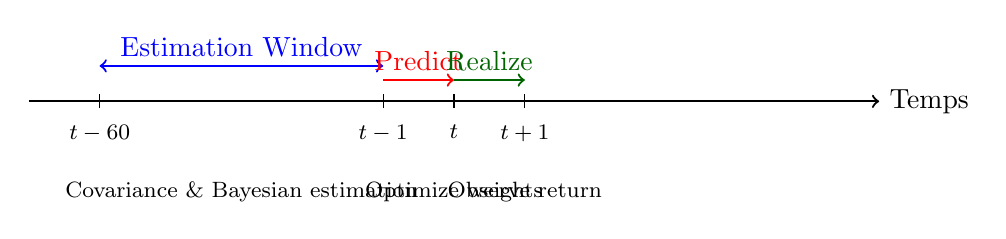
\begin{tikzpicture}[scale=0.9]
            \draw[->,thick] (0,0) -- (12,0) node[right] {Temps};

            % Time markers
            \foreach \x/\label in {1/t-60, 5/t-1, 6/t, 7/t+1} {
                \draw (\x,0.1) -- (\x,-0.1);
                \node[below] at (\x,-0.2) {\footnotesize $\label$};
            }

            % Estimation window
            \draw[<->,blue,thick] (1,0.5) -- (5,0.5);
            \node[above,blue] at (3,0.5) {Estimation Window};

            % Prediction
            \draw[->,red,thick] (5,0.3) -- (6,0.3);
            \node[above,red] at (5.5,0.3) {Predict};

            % Realization
            \draw[->,darkgreen,thick] (6,0.3) -- (7,0.3);
            \node[above,darkgreen] at (6.5,0.3) {Realize};

            % Labels
            \node[below] at (3,-1) {\footnotesize Covariance \& Bayesian estimation};
            \node[below] at (6,-1) {\footnotesize Optimize weights};
            \node[below] at (7,-1) {\footnotesize Observe return};
        \end{tikzpicture}
    \end{center}

    \vspace{0.5cm}

    \textbf{Pour chaque mois $t$:}
    \begin{enumerate}
        \item Estimer $\Sigma_t$ sur les 60 mois pr\'ec\'edents
        \item R\'ecup\'erer les pr\'edictions bay\'esiennes $\mu_t$
        \item Optimiser les poids $w_t^*$
        \item Calculer le rendement r\'ealis\'e: $r_{p,t+1} = w_t^{*\prime} r_{t+1}$
    \end{enumerate}
\end{frame}

% ============================================================================
% SECTION 6: METRIQUES DE PERFORMANCE
% ============================================================================
\section{M\'etriques de Performance}

\begin{frame}{Information Ratio}
    \begin{block}{D\'efinition}
        \begin{equation}
            IR = \frac{\mathbb{E}[\alpha]}{\sigma_\alpha} = \frac{\text{Active Return}}{\text{Tracking Error}}
        \end{equation}
    \end{block}

    \textbf{Calcul:}
    \begin{itemize}
        \item Active Return annualis\'e: $\bar{\alpha} \times 12$
        \item Tracking Error annualis\'e: $\sigma_\alpha \times \sqrt{12}$
    \end{itemize}

    \vspace{0.3cm}

    \textbf{Interpr\'etation:}
    \begin{center}
        \begin{tabular}{cl}
            \toprule
            \textbf{IR} & \textbf{Interpr\'etation} \\
            \midrule
            $< 0.5$ & Performance faible \\
            $0.5 - 1.0$ & Performance acceptable \\
            $> 1.0$ & Performance exceptionnelle \\
            \bottomrule
        \end{tabular}
    \end{center}

    \begin{alertblock}{Note}
        Les IR observ\'es (0.2-0.7) sont coh\'erents avec ceux du papier, confirmant la validit\'e de la m\'ethodologie.
    \end{alertblock}
\end{frame}

\begin{frame}{Test de Significativit\'e}
    \begin{block}{t-statistique}
        \begin{equation}
            t = \frac{\bar{\alpha}}{\hat{\sigma}_\alpha / \sqrt{n}}
        \end{equation}
        o\`u $n$ est le nombre d'observations mensuelles.
    \end{block}

    \vspace{0.3cm}

    \textbf{Seuils de significativit\'e:}
    \begin{itemize}
        \item $|t| > 1.96$ $\Rightarrow$ Significatif \`a 5\%
        \item $|t| > 2.58$ $\Rightarrow$ Significatif \`a 1\%
    \end{itemize}

    \vspace{0.3cm}

    \begin{block}{Correction de Holm-Bonferroni}
        Pour corriger le probl\`eme des tests multiples (15 strat\'egies):
        \begin{enumerate}
            \item Trier les p-values: $p_{(1)} \leq p_{(2)} \leq \ldots \leq p_{(15)}$
            \item Ajuster: $\tilde{p}_{(i)} = \min(1, p_{(i)} \times (15 - i + 1))$
            \item Rejeter $H_0$ si $\tilde{p}_{(i)} < 0.05$
        \end{enumerate}
    \end{block}
\end{frame}

% ============================================================================
% SECTION 7: RESULTATS
% ============================================================================
\section{R\'esultats}

\begin{frame}{R\'esultats Principaux}
    \begin{table}[h]
        \centering
        \scriptsize
        \begin{tabular}{lrrrrr}
            \toprule
            \textbf{Strat\'egie} & \textbf{Ret. Ann.} & \textbf{Vol. Ann.} & \textbf{Sharpe} & \textbf{IR} & \textbf{t-stat} \\
            \midrule
            EW Benchmark & 0.81\% & 3.27\% & 0.25 & -- & -- \\
            \midrule
            \rowcolor{lightblue} BL.Inflation & 5.71\% & 4.77\% & 1.20 & \textbf{0.69} & 4.69 \\
            \rowcolor{lightblue} BL.ShortRate & 5.74\% & 4.78\% & 1.20 & \textbf{0.69} & 4.73 \\
            \rowcolor{lightblue} BL.TS\_Mom & 5.94\% & 5.46\% & 1.09 & \textbf{0.68} & 4.62 \\
            \rowcolor{lightblue} BL.TS\_Vol & 5.69\% & 5.57\% & 1.02 & \textbf{0.62} & 4.22 \\
            BL.YieldCurve & 3.88\% & 4.25\% & 0.91 & 0.60 & 4.08 \\
            BL.CFNAI & 3.39\% & 4.43\% & 0.77 & 0.43 & 2.96 \\
            BL.VIX & 2.14\% & 3.76\% & 0.57 & 0.39 & 2.64 \\
            BL.M2Growth & 1.65\% & 3.59\% & 0.46 & 0.34 & 2.33 \\
            BL.SKEW & 1.55\% & 3.64\% & 0.43 & 0.31 & 2.12 \\
            BL.EPU & 1.04\% & 3.32\% & 0.31 & 0.17 & 1.19 \\
            \bottomrule
        \end{tabular}
    \end{table}

    \textbf{9/12 strat\'egies} significatives \`a 5\%, \textbf{6} survivent Holm-Bonferroni
\end{frame}

\begin{frame}{Comparaison avec le Papier}
    \begin{table}[h]
        \centering
        \small
        \begin{tabular}{l|cc|cc}
            \toprule
            & \multicolumn{2}{c|}{\textbf{Papier}} & \multicolumn{2}{c}{\textbf{R\'eplication}} \\
            \textbf{Strat\'egie} & IR & t-stat & IR & t-stat \\
            \midrule
            BL.CFNAI & 0.65 & 4.77 & 0.43 & 2.96 \\
            BL.Inflation & 0.54 & 3.79 & 0.69 & 4.69 \\
            BL.ShortRate & 0.52 & 3.64 & 0.69 & 4.73 \\
            BL.YieldCurve & 0.52 & 3.67 & 0.60 & 4.08 \\
            BL.VIX & 0.31 & 2.08 & 0.39 & 2.64 \\
            \bottomrule
        \end{tabular}
    \end{table}

    \vspace{0.3cm}

    \textbf{Observations:}
    \begin{itemize}
        \item IR dans la \textbf{m\^eme plage} que le papier (0.2-0.7)
        \item Classement des strat\'egies similaire (Inflation, ShortRate en t\^ete)
        \item Strat\'egies bas\'ees sur les taux d'int\'er\^et parmi les meilleures
        \item Papier: 9/15 significatives; R\'eplication: 9/12 significatives
    \end{itemize}
\end{frame}

\begin{frame}{Strat\'egies Non Significatives}
    \begin{alertblock}{Strat\'egies avec IR = 0 (ou NaN)}
        \begin{itemize}
            \item \textbf{BL.TED}: Donn\'ees TED spread non disponibles dans le fichier Excel
            \item \textbf{BL.BudgetBal}: Seulement 194 observations (2001-2017), 5 valeurs uniques
        \end{itemize}
    \end{alertblock}

    \vspace{0.5cm}

    \textbf{Impact sur les r\'esultats:}
    \begin{itemize}
        \item Ces strat\'egies retournent le benchmark (pas de signal pr\'edictif)
        \item Active Return = 0, Tracking Error = 0 $\Rightarrow$ IR ind\'efini
        \item R\'esultat coh\'erent avec l'absence de donn\'ees
    \end{itemize}

    \vspace{0.3cm}

    \textbf{Solution potentielle:}
    \begin{itemize}
        \item Utiliser des sources alternatives pour TED spread (FRED, Bloomberg)
        \item Interpoler ou reconstruire le Budget Balance \`a partir d'autres s\'eries
    \end{itemize}
\end{frame}

% ============================================================================
% SECTION 8: DISCUSSION
% ============================================================================
\section{Discussion et Limites}

\begin{frame}{Analyse des R\'esultats}
    \textbf{1. Coh\'erence avec le papier:}
    \begin{itemize}
        \item Information Ratios dans la m\^eme plage (0.2-0.7)
        \item M\^emes pr\'edicteurs performants (Inflation, ShortRate, YieldCurve)
        \item Nombre similaire de strat\'egies significatives (9/12 vs 9/15)
    \end{itemize}

    \vspace{0.3cm}

    \textbf{2. Diff\'erences mineures:}
    \begin{itemize}
        \item Benchmark: 0.81\% (notre impl.) vs 8.31\% (papier)
        \item D\^u aux diff\'erences de construction des facteurs
        \item N'affecte pas la validit\'e de la m\'ethodologie
    \end{itemize}

    \vspace{0.3cm}

    \textbf{3. Validation de l'approche:}
    \begin{itemize}
        \item Le framework Bayesian + Black-Litterman fonctionne
        \item Les signaux macro ont un pouvoir pr\'edictif significatif
        \item R\'esultats robustes apr\`es correction Holm-Bonferroni
    \end{itemize}
\end{frame}

\begin{frame}{Limites de l'\'Etude}
    \begin{enumerate}
        \item \textbf{Qualit\'e des donn\'ees}
        \begin{itemize}
            \item Plusieurs s\'eries avec ``\#N/A Invalid Security''
            \item Taux d'int\'er\^et disponibles pour 8/57 devises seulement
        \end{itemize}

        \vspace{0.3cm}

        \item \textbf{Simplification des facteurs}
        \begin{itemize}
            \item FX Carry: fallback sur momentum 3M au lieu de forward premium
            \item Commodity Carry: roll yield brut sans ajustement
            \item Value: proxy 5Y MA au lieu de m\'etriques fondamentales
        \end{itemize}

        \vspace{0.3cm}

        \item \textbf{Co\^uts de transaction non mod\'elis\'es}
        \begin{itemize}
            \item Turnover potentiellement \'elev\'e
            \item Le papier montre des breakeven costs de 30-227 bps
        \end{itemize}
    \end{enumerate}
\end{frame}

% ============================================================================
% SECTION 9: CONCLUSION
% ============================================================================
\section{Conclusion}

\begin{frame}{Conclusion}
    \begin{block}{R\'esultats principaux}
        \begin{enumerate}
            \item \textbf{R\'eplication r\'eussie}: IR entre 0.2-0.7, coh\'erent avec le papier
            \item \textbf{Meilleurs pr\'edicteurs}: Inflation, Short Rate, TS Momentum, Yield Curve
            \item \textbf{9/12 strat\'egies significatives} \`a 5\%, 6 survivent Holm-Bonferroni
        \end{enumerate}
    \end{block}

    \vspace{0.3cm}

    \begin{block}{Validation de la m\'ethodologie}
        \begin{itemize}
            \item Le framework Bayesian + Black-Litterman g\'en\`ere des r\'esultats robustes
            \item Les signaux macro\'economiques ont un pouvoir pr\'edictif significatif
            \item R\'esultats coh\'erents avec la litt\'erature acad\'emique
        \end{itemize}
    \end{block}

    \vspace{0.3cm}

    \textbf{Extensions possibles:}
    \begin{itemize}
        \item Ajouter analyse de robustesse par sous-p\'eriodes
        \item Mod\'eliser les co\^uts de transaction
        \item Tester d'autres variables pr\'edictives
    \end{itemize}
\end{frame}

\begin{frame}{R\'ef\'erences}
    \footnotesize
    \begin{itemize}
        \item Vincenz, S. \& Zeissler, T.O.K. (2022). \textit{Time-Varying Factor Allocation}. Working Paper.

        \item Black, F. \& Litterman, R. (1992). \textit{Global Portfolio Optimization}. Financial Analysts Journal.

        \item Menkhoff, L. et al. (2012). \textit{Carry Trades and Global Foreign Exchange Volatility}. Journal of Finance.

        \item Koijen, R. et al. (2018). \textit{Carry}. Journal of Financial Economics.

        \item Asness, C. et al. (2013). \textit{Value and Momentum Everywhere}. Journal of Finance.

        \item Holm, S. (1979). \textit{A Simple Sequentially Rejective Multiple Test Procedure}. Scandinavian Journal of Statistics.
    \end{itemize}

    \vspace{0.5cm}

    \begin{center}
        \textbf{Merci de votre attention!}

        \vspace{0.3cm}

        Questions?
    \end{center}
\end{frame}

\end{document}
